\documentclass{siamltex}

% Include useful packages
\usepackage{fullpage}
\usepackage{graphicx}
\usepackage{amsmath}
\usepackage{amssymb}
\usepackage{amsfonts}
\usepackage{color} 
\usepackage{fancyvrb}
\usepackage[sort, numbers]{natbib}
\usepackage{url}

\linespread{1.4}

% Helpful commands for mathematical expressions
\newcommand{\dd}[2]{\dfrac{\textrm{d} #1}{\textrm{d} #2}}
\newcommand{\pdd}[2]{\dfrac{\partial#1}{\partial#2}}
\newcommand{\pddb}[2]{\left( \dfrac{\partial#1}{\partial#2} \right)}
\newcommand{\boldnabla}{\mbox{\boldmath$\nabla$}}
\renewcommand{\vec}[1]{\mathbf{#1}}
\newcommand{\uvec}[1]{\mathbf{#1}}
%\renewcommand{\and}{ \text{and} }
\newcommand{\for}{ \text{for} }

% Helpful commands for authors' notes
%\newcommand{\completed}{[Completed]}
%\newcommand{\todo}{[Started]}
%\newcommand{\tostart}{[Still to do]}
\newcommand{\authornote}[2]{{\bf [#1: #2]}}
\newcommand{\alex}[1]{\authornote{Alex}{#1}}
\newcommand{\ozzy}[1]{\authornote{Ozzy}{#1}}
\newcommand{\highlight}[1]{{\color{red} \bf{#1}}}

\begin{document}

% Make title

\title{The influence of cell-based modelling paradigm on the outcome of multiscale simulations of cell populations}

\author{J.M. Osborne\footnotemark[2]\ \footnotemark[4]\ \thanks{Corresponding author ({\tt James.Osborne@cs.ox.ac.uk})}\ \and A.G. Fletcher\footnotemark[3]\ \footnotemark[4] \and OTHER AUTHORS\and P.K. Maini\footnotemark[3] \and D.J. Gavaghan\footnotemark[2]}

\renewcommand{\thefootnote}{\fnsymbol{footnote}}
\footnotetext[2]{Computational Biology Group, Department of Computer Science, Wolfson Building, Parks Road, Oxford OX1 3QD, UK}
\footnotetext[3]{Centre for Mathematical Biology, Mathematical Institute, 24-29 St Giles', Oxford OX1 3LB, UK}
\footnotetext[4]{Joint first authors}
\renewcommand{\thefootnote}{\arabic{footnote}}

% Notice that the footnote marks begin with [2] because the first mark (the asterisk) will be used in the title for date-recieved information by SIAM, even if not already used for support data.

%\ead{alexander.fletcher@maths.ox.ac.uk}
%\cortext[cor1]{Corresponding author}
%\fntext[fn1]{Joint first authors}

\maketitle

\begin{abstract}
The key results intended for this paper are: a comparison of different cell-level modelling approaches (cellular Potts model, centre dynamics models and vertex dynamics models); a brief discussion of the implementation of these approaches within the Chaste framework; and a comparison of the different Chaste codes used to create example simulations. 

\highlight{Some notes:
\begin{itemize}
\item We will aim to submit this manuscript to Multiscale Modeling and Simulation: A SIAM Interdisciplinary Journal, so need to check that journal's submission requirements.
\item We need to carefully define what is novel in this paper, and what will have already been covered in the other recent Chaste papers.
\item Once a rough first draft is in place, we should send round to people and decide on authorship: presumably, those developers that have helped to develop the cell-based functionality exhibited in this paper.
\item We need to ensure consistency in naming and terminology throughout, e.g. `cell-based model' versus `individual-based model'.
\item This based upcoming 3.1 release due to including recent functionality.
\item See also \tt{https://chaste.cs.ox.ac.uk/cgi-bin/trac.cgi/wiki/CellBasedComparisonPaper}.
\end{itemize}
}
\end{abstract}

\begin{keywords}
\highlight{To do}
\end{keywords}

\begin{AMS}
\highlight{To do}
\end{AMS}


%%%%%%%%%%%%%%%%%%%%%%%%%%%%%%%%%%%%%%%%%%%%%%%%%%
%%%%%%%%%%%%%%%%%%%% Section %%%%%%%%%%%%%%%%%%%%%
%%%%%%%%%%%%%%%%%%%%%%%%%%%%%%%%%%%%%%%%%%%%%%%%%%
\section{Introduction} \label{sec1}

\subsection{A short review of cell-based models}

\begin{itemize}
\item Conclude by discussing recent multiscale models, which couple the biomechanical behaviour of a cell aggregate or tissue to other processes such as fluid or solute transport.
\end{itemize}

\subsection{Where models come from}

\subsection{Simulation methods}

\begin{itemize}
\item Deterministic: solving equations of motion.
\item Stochastic: (a)synchronous updating; Gillespie algorithm and variations; Monte Carlo simulation.
\item Hybrid simulations.
\end{itemize}

\subsection{Comparing models; why we need a consistent simulation framework}

\begin{itemize}
\item Technical considerations.
\item To date there has been very little comparative study of different cell-based modelling paradigms.
\item Clearly, each approach has general strengths and weaknesses (see next section for further details).
\item To what extent are the results of model simulations artifacts of the modelling approach used or method of simulation?
\item It is difficult to make an accurate quantitative comparison between different models and thus assess the influence of mode choice on the behaviour of simulations.
\item This difficulty is compounded in hybrid or multiscale models.
\item If we use a consistent computational framework within which to simulate these models, then we can compare different constitutive assumptions by altering model details in a straightforward manner.
\end{itemize}

\highlight{What other attempts have been made to compare different models? By us \cite{Osborne2010Hybrid} as well as others.}

The remainder of this paper is structured as follows...

%%%%%%%%%%%%%%%%%%%%%%%%%%%%%%%%%%%%%%%%%%%%%%%%%%
%%%%%%%%%%%%%%%%%%%% Section %%%%%%%%%%%%%%%%%%%%%
%%%%%%%%%%%%%%%%%%%%%%%%%%%%%%%%%%%%%%%%%%%%%%%%%%
\section{Cell-based models of biological tissues}\label{sec:discrete_models}
The multiscale modelling framework consists of three main interacting scales: the cellular scale; the subcellular scale; and the tissue scale.

\highlight{We need to make some kind of justification for this distinction of spatial scales. Who first did this, from a modelling point of view? Clarify that we know that, really, biology is the integration of these processes but that this framework seems like a resonable way forward.}

%%%%%%%%%%%%%%%%%%% SubSection %%%%%%%%%%%%%%%%%%%
\subsection{Discrete representations of cells} \label{sec:cell_level}
Various different model for interacting populations of cells have been proposed. The main ones are given here.

\highlight{This section should contain all the mathematics of the models. Not the full detail as can refernce papers but enought to give a feel for similarities and differences. This text is availiable in Ozzy's thesis and Junked sections from older papers.}


\highlight{Go through each of the modelling approaches listed below and provide a brief overview. 
Typical biological systems studied with each model, with relevant references, and give some details of the underlying equations, geometric representation, etc. Dont discuss coupling with other scales till next section.}

\begin{description}
	\item [Cellular Automata.]
	{The simplest form of cellular modelling, cells are represented as points on a lattice and rules constructed in order for each cell to divide, move or die. 
    Cells can only divide in to neighbouring spaces on the lattice. 
    Some of the issues with this type of modelling include: effects felt at distance; fixed regular lattice geometry; growth is lattice dependent -- 4 point $\rightarrow$ star and 8 point $\rightarrow$ octagon; and finally you can't consider stress in the tissue.}

	\item [Cellular Potts.]
	{An extension of cellular automata model is the Cellular Potts Model, in which cells are composed of a number of lattice points, and the cell shape is evolved by minimizing the energy which is calculated by imposing constraints due to chemotaxis etc. 
	This form of modelling is utilised in the CompuCell3D modelling package produced at Indiana University. 
	\highlight{ - can we refer to the `Potts in Chaste' paper here should be submitted before this.}}

    \item [Overlapping sphere models.]
    {See the work of Drasdo \emph{et al}, for example \citep{Drasdo2007Role}.
    Cells are modelled as overlapping spheres and energy minimization is used to evolve the system, cells can divide depending on binary rules or by using a cell cycle model. 		
    The software package MASON from UCSF deals with this type of modelling. 
    Extensions include ellipses with varying radii and orientation [REF]. 
    Chaste functionality for this is discussed in a recent computational study by \citet{Pathmanathan2009Computational} of the mechanical properties of this class of model.}

    \item [Subcellular Element Model.]
    {This is an extension of the overlapping spheres approach and treats cells as being composed of subcellular elements with different interactions between inter-cell and intra-cell elements \citep{Newman2005Modeling,Sandersius2008Modeling} }

    \item[Centre Dynamics Tessellation Models.] 
    {This was the first class of cell-based model added to Chaste \citep{Leeuwen2009Integrative} and are based on the model presented by \citet{Meineke2001Cell}.}

    \item[Vertex Dynamics Models.] 
    {Cells defined by polygons and movement determined by energy minimization. Currently implemented in Chaste in two dimensions \citep{Osborne2010Hybrid}. 
    \highlight{ - hopefully refer to our vertex paper here!}}

    \item[Finite Element Models.] 
    {Generalization of vertex where cell represented as collections of moving and deforming elements -- tetrahedra for example.}	

\end{description}

%%%%%%%%%%%%%%%%%%% SubSection %%%%%%%%%%%%%%%%%%%
\subsection{Coupling to other scales} \label{sec:scales}

\begin{description}
    \item [The subcellular (micro) scale.] 
    {The behaviour of cells is dictated by modelling the numerous subcellular processes occurring within the cell. 
    The main modelling paradigm is to use reaction networks rendered into ODEs which interacting with cell level through the cell cycle and also directly through properties such as cell size, shape and motility etc. 
    Other methods include: stochastic ODEs; PDEs; or fully stochastic networks which represent the transport and use of substrates within cells.}

    \item [The tissue (macro) scale.] 
    {Modelling of inter-cellular signalling, or nutrient transfer can be considered by using reaction diffusion equations, which are solved on the growing domain (defined by the cells) with cells acting as sinks and sources \ozzy{We don't have PDEs for vertex yet: we should reference Aaron's paper here \citep{Smith2011Incorporating}}.}
\end{description}

The advantage of such a framework is that once you have implemented a particular subcellular model you can use it in all possible cell level models.

%%%%%%%%%%%%%%%%%%%%%%%%%%%%%%%%%%%%%%%%%%%%%%%%%%
%%%%%%%%%%%%%%%%%%%% Section %%%%%%%%%%%%%%%%%%%%%
%%%%%%%%%%%%%%%%%%%%%%%%%%%%%%%%%%%%%%%%%%%%%%%%%%
\section{Computational structure} \label{sec:computational_structure}


\subsection{Chaste} \label{sec:chaste} 
Chaste (Cancer, Heart and Soft Tissue Environment) is a collaborative software development project, which is designed to act as a high-quality multi-purpose library supporting computational simulations for a wide range of biological problems \citep{Pitt-Francis2008Chaste}. 
In this context, ‘high-quality’ means that the software is extensible, robust, fast, accurate and maintainable and uses state-of-the-art numerical techniques. 
It is also open-source, so can be adapted by other developers. 
Chaste has been developed by a multidisciplinary team including mathematicians and software engineers. 
This ensures that the code is well-structured as a piece of software, while at the same time practical and useful as a computational modelling tool. 
While it is a generic extensible library, to date attention has focused on the fields of cardiac electrophysiology and tumor growth \citep{Pitt-Francis2009Chaste}. 
Further details on Chaste are available at \url{http://www.cs.ox.ac.uk/chaste}. 

The Cell Based component of Chaste utilises the core functionality of Chaste detailed in \citep{Pitt-Francis2009Chaste}, but contains a number of specific classes which implement the models duiscussed in Section~\ref{sec:discrete_models}.

% I think we would be better off leaving this level of detail  to the CPC paper
%\begin{figure}[tbhp]
%        \centering
%        \setlength{\unitlength}{1cm}
%        \begin{picture}(10,10)
%              \put(0,0){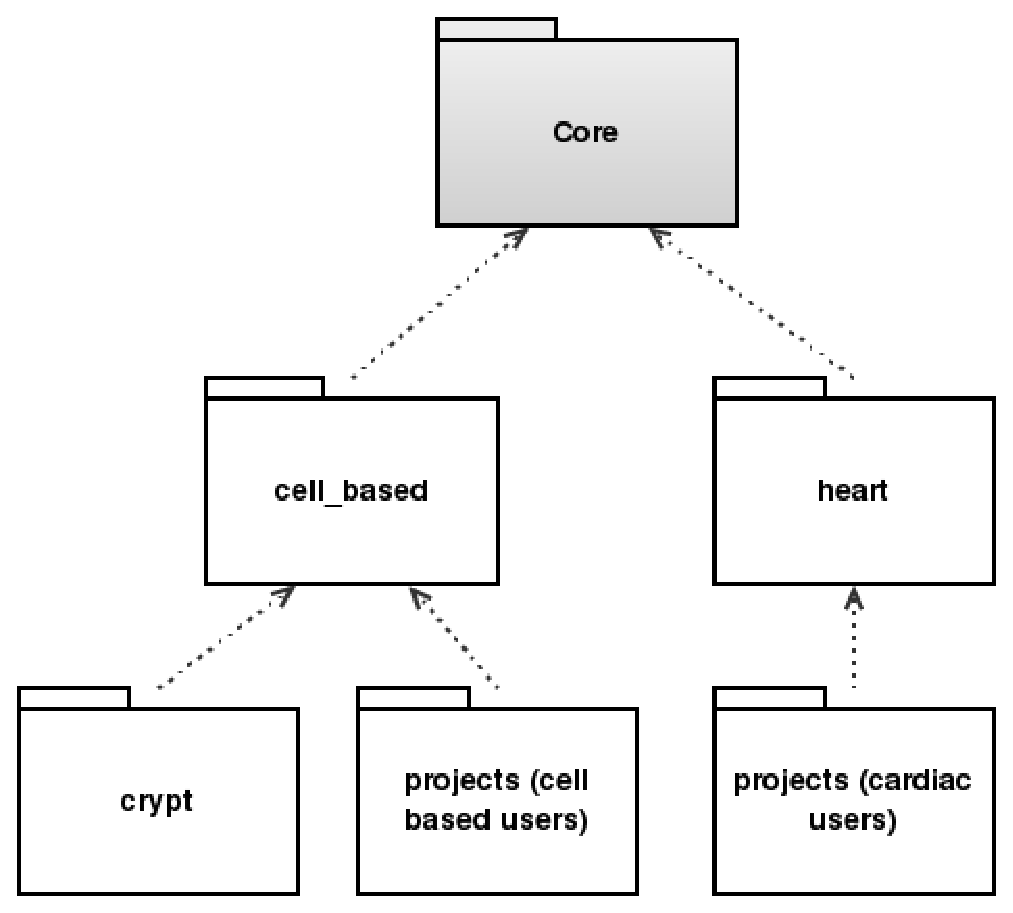
\includegraphics[width=10cm]{Figs/ChasteStructure}}
%	      \put(1.5,5.0){\huge{Need to change this and}}
%              \put(0.0,3.5){\huge{add Crypt and projects folders.}}
%        \end{picture}
%        \caption{Schematic diagram of Chaste code base.} 
%       \label{fig:ChasteStructure}
%\end{figure}

%%%%%%%%%%%%%%%%%%% SubSection %%%%%%%%%%%%%%%%%%%
\subsection{Structure of code} \label{sec:code}
To set up a cell-based simulation within Chaste you need to instantiate a collection of objects, which specify the properties of the simulation. 
The following eight objects can be defined for a simulation to be undertaken: \textbf{Mesh; Cells; Cell Population; Simulation; Forces/ Update Rules; *Cell Killers; *Boundary Conditions (BCS); and *External Factors}.
The starred objects are optional as you may not want to have cells being removed from the simulation and the growth may be unconstrained. Technicaly Forces and Update rules are optional as a simulation will run without them and cells can divide and die, however the cells will not move.

\begin{figure}[tbhp]
        \centering
        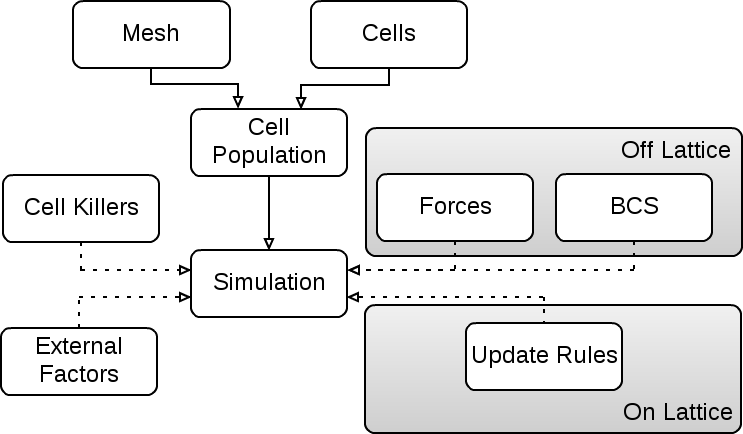
\includegraphics[width=10cm]{Figs/CellBasedStructure}
        \caption{Schematic diagram of the framework showing the separate components of the simulations and the communication between the classes. Necesary inclusions are illustrated by solid lines and optional ones are denoted by dashed lines} 
       \label{fig:SimulationComponents}
\end{figure}

In the following sections we detail each of these components and how they relate to elemets of the simulatiosn discussed in Section~\ref{sec:discrete_models}. \highlight{Go through these sections and add more detail including the links beween them.}

%%%%%%%%%%%%%%%%%%% SubSection %%%%%%%%%%%%%%%%%%%
\subsection{Mesh} \label{sec:structure:mesh}
The structural information for the simulation, for example the initial epithelial layer layout is defined here.

%%%%%%%%%%%%%%%%%%% SubSection %%%%%%%%%%%%%%%%%%%
\subsection{Cells} \label{sec:structure:cells}
A collection of cells to be associated with the mesh. 
Contain all the subcellular machinery. 
The initial conditions for  subcellular models are defined here.

These are cell-level model independent.

%%%%%%%%%%%%%%%%%%% SubSection %%%%%%%%%%%%%%%%%%%
\subsection{Cell Population} \label{sec:structure:cell_pop}
Associates the cells with the mesh and provides a mechanism for cells to know their location.

%%%%%%%%%%%%%%%%%%% SubSection %%%%%%%%%%%%%%%%%%%
\subsection{Simulation} \label{sec:structure:simulation}
Takes in the cell population and implements the rules for evolution of the system.
Also takes in the remaining objects to specify details of the simulation.
Evolves the system through time.

There are on- and off-lattice specific classes.

%%%%%%%%%%%%%%%%%%% SubSection %%%%%%%%%%%%%%%%%%%
\subsection{Forces / Update Rules} \label{sec:structure:updates}
These are passed in to the simulation and dictate the way the cells move.
In off lattice simulations \texttt{Forces} dictate how the nodes move.
In on lattice simulations \texttt{UpdateRules} define the probability of acepting a proposed conformational change (i.e. movement).
Subclasses of specific models can be implemented using different \texttt{Forces} or \texttt{UpdateRules} and multiple rules can be used to model different biological processes.


%%%%%%%%%%%%%%%%%%% SubSection %%%%%%%%%%%%%%%%%%%
\subsection{Cell Killers} \label{sec:structure:cell_killers}
These are passed to the simulation and define how cells die and are removed from the simulation. 
Multiple killers can be used at the same time for example to represent random death and death due to sloughing.

These are cell-level model independent.


%%%%%%%%%%%%%%%%%%% SubSection %%%%%%%%%%%%%%%%%%%
\subsection{Boundary Conditions} \label{sec:structure:bcs}
These are passed to the simulation and define any fixed restrictions on how the cells can move. 
Multiple conditions can be used at the same time.
Note that these are only use in off-lattice simulations as domain restrictions are implicitly defined in the mesh when using an on-lattice model.


%%%%%%%%%%%%%%%%%%% SubSection %%%%%%%%%%%%%%%%%%%
\subsection{External Factors} \label{sec:structure:external}
These are passed to the simulation and define any external factors for example imposed gradients or the diffusion an uptake (secretion) of metabolites.

These are cell-level model independent.



In order to create and run a simulation these objects are combined together. To show how this works we now present a series of example simulations using chaste. In addition we will use these examples to compare and contrast the different cell-level models.


%%%%%%%%%%%%%%%%%%%%%%%%%%%%%%%%%%%%%%%%%%%%%%%%%%
%%%%%%%%%%%%%%%%%%%% Section %%%%%%%%%%%%%%%%%%%%%
%%%%%%%%%%%%%%%%%%%%%%%%%%%%%%%%%%%%%%%%%%%%%%%%%%
\section{Example simulations} \label{sec:example_simulations}

The simulations to be undertaken are...

\noindent Will have all Potts Mesh Node and Vertex-Based simulations:
\begin{itemize}
  \item Monolayer \highlight{- if background needed, we can add some text from AGF thesis and some text that was cut out of the vertex paper}
  \item crypt \highlight{- what will be novel, i.e. how will we progress beyond \citet{Osborne2010Hybrid} in our comparison? 1) Have all 4 models 2) show how it evolves from Monolayer.}
\end{itemize}
All but Vertex
\begin{itemize}
  \item Spheroid \highlight{- if background needed, we can add some text from AGF thesis}
\end{itemize}
Will only have Vertex and Potts
\begin{itemize}
  \item Cell sorting, in vertex and Potts \highlight{Will  be discussing }
\end{itemize}
Only node based and Potts
\begin{itemize}
  \item 3D Crypt. \highlight{Can reference SJ and Ozzy crypt paper if out?}
\end{itemize}


%%%%%%%%%%%%%%%%%%% SubSection %%%%%%%%%%%%%%%%%%%
\subsection{Demonstration of growing monolayer} \label{sec:growing_domain}
\begin{itemize}
  \item Demonstrate basic functionality
  \item Example of growing monolayer with void removal, sloughing? etc. 
  \item Show differences in code from model to model
  \item Make sure to differntiate from simple example in CPC part Deux
\end{itemize}
\begin{small}
\begin{Verbatim}[frame=single, numbers=left, numbersep=2pt]
void TestVertexMonolayerWithRandomBirthAndDeath() throw (Exception)
{
    // Create a simple 2D vertex mesh
    HoneycombVertexMeshGenerator generator(5, 5);
    MutableVertexMesh<2,2>* p_mesh = generator.GetMesh();

    // Set up cells, one for each element in the vertex mesh
    std:vector<CellPtr> cells;
    CellsGenerator<StochasticDurationGenerationBasedCellCycleModel, 2>
        cells_generator;
    cells_generator.GenerateBasic(cells,p_mesh->GetNumElements());

    // Create cell population
    VertexBasedCellPopulation<2> cell_population(*p_mesh, cells);

    // Set up cell-based simulation
    CellBasedSimulation<2> simulator(cell_population);
    simulator.SetOutputDirectory("TestVertexMonolayer");
    simulator.SetEndTime(40);

    // Create a force law and pass it to the simulation
    NagaiHondaForce<2> force_law;
    simulator.AddForce(&force_law);

    // Create cell killer and pass it to the simulation
    RandomCellKiller<2> random_cell_killer(&cell_population, 0.01);
    simulator.AddCellKiller(&random_cell_killer);

    // Run simulation
    simulator.Solve();
}
\end{Verbatim}
\end{small}

%%%%%%%%%%%%%%%%%%% SubSection %%%%%%%%%%%%%%%%%%%
\subsection{Demonstration of cell sorting} \label{sec:cell_sorting}
\begin{itemize}
 \item Potts and Vertex comparison. \highlight{we can add some text that was cut out of the vertex paper}
\end{itemize}

%%%%%%%%%%%%%%%%%%% SubSection %%%%%%%%%%%%%%%%%%%
\subsection{Demonstration of spheroid} \label{sec:spheroid}
\begin{itemize}
 \item Include nutrient diffusion. \highlight{Talk about Dan's stuff; this example illustrates PDE handling.}
\end{itemize}

%%%%%%%%%%%%%%%%%%% SubSection %%%%%%%%%%%%%%%%%%%
\subsection{Demonstration of crypt} \label{sec:crypt}
\begin{itemize}
  \item 2D cylindrical crypt in each modality. 
  \item 3D node-based crypt.
  \item Sara-Jane's work?
\end{itemize}


%%%%%%%%%%%%%%%%%%%%%%%%%%%%%%%%%%%%%%%%%%%%%%%%%%
%%%%%%%%%%%%%%%%%%%% Section %%%%%%%%%%%%%%%%%%%%%
%%%%%%%%%%%%%%%%%%%%%%%%%%%%%%%%%%%%%%%%%%%%%%%%%%
\section{Discussion} \label{sec:discussion}

%%%%%%%%%%%%%%%%%%%%%%%%%%%%%%%%%%%%%%%%%%%%%%%%%%
%%%%%%%%%%%%%%%%%%%% Section %%%%%%%%%%%%%%%%%%%%%
%%%%%%%%%%%%%%%%%%%%%%%%%%%%%%%%%%%%%%%%%%%%%%%%%%
\section*{Acknowledgements}

JMO is supported by the Life Sciences Interface and Systems Biology Doctoral Training Centres (EP/E501605/1 and EP/G50029/1 respectively) and Microsoft Research, Cambridge. 
AGF is supported by EPSRC (EP/I017909/1) and Microsoft Research, Cambridge. 
\highlight{Add acknowledgements from any other authors.}

\clearpage

%%%%%%%%%%%%%%%%%%%%%%%%%%%%%%%%%%%%%%%%%%%%%%%%%%
%%%%%%%%%%%%%%%%%%%% Section %%%%%%%%%%%%%%%%%%%%%
%%%%%%%%%%%%%%%%%%%%%%%%%%%%%%%%%%%%%%%%%%%%%%%%%%
\bibliography{comparison_refs}{}
\bibliographystyle{apalike}

\end{document}
